\documentclass[twoside]{book}

% Packages required by doxygen
\usepackage{fixltx2e}
\usepackage{calc}
\usepackage{doxygen}
\usepackage[export]{adjustbox} % also loads graphicx
\usepackage{graphicx}
\usepackage[utf8]{inputenc}
\usepackage{makeidx}
\usepackage{multicol}
\usepackage{multirow}
\PassOptionsToPackage{warn}{textcomp}
\usepackage{textcomp}
\usepackage[nointegrals]{wasysym}
\usepackage[table]{xcolor}

% NLS support packages
\usepackage{polski}
\usepackage[T1]{fontenc}

% Font selection
\usepackage[T1]{fontenc}
\usepackage[scaled=.90]{helvet}
\usepackage{courier}
\usepackage{amssymb}
\usepackage{sectsty}
\renewcommand{\familydefault}{\sfdefault}
\allsectionsfont{%
  \fontseries{bc}\selectfont%
  \color{darkgray}%
}
\renewcommand{\DoxyLabelFont}{%
  \fontseries{bc}\selectfont%
  \color{darkgray}%
}
\newcommand{\+}{\discretionary{\mbox{\scriptsize$\hookleftarrow$}}{}{}}

% Page & text layout
\usepackage{geometry}
\geometry{%
  a4paper,%
  top=2.5cm,%
  bottom=2.5cm,%
  left=2.5cm,%
  right=2.5cm%
}
\tolerance=750
\hfuzz=15pt
\hbadness=750
\setlength{\emergencystretch}{15pt}
\setlength{\parindent}{0cm}
\setlength{\parskip}{3ex plus 2ex minus 2ex}
\makeatletter
\renewcommand{\paragraph}{%
  \@startsection{paragraph}{4}{0ex}{-1.0ex}{1.0ex}{%
    \normalfont\normalsize\bfseries\SS@parafont%
  }%
}
\renewcommand{\subparagraph}{%
  \@startsection{subparagraph}{5}{0ex}{-1.0ex}{1.0ex}{%
    \normalfont\normalsize\bfseries\SS@subparafont%
  }%
}
\makeatother

% Headers & footers
\usepackage{fancyhdr}
\pagestyle{fancyplain}
\fancyhead[LE]{\fancyplain{}{\bfseries\thepage}}
\fancyhead[CE]{\fancyplain{}{}}
\fancyhead[RE]{\fancyplain{}{\bfseries\leftmark}}
\fancyhead[LO]{\fancyplain{}{\bfseries\rightmark}}
\fancyhead[CO]{\fancyplain{}{}}
\fancyhead[RO]{\fancyplain{}{\bfseries\thepage}}
\fancyfoot[LE]{\fancyplain{}{}}
\fancyfoot[CE]{\fancyplain{}{}}
\fancyfoot[RE]{\fancyplain{}{\bfseries\scriptsize Wygenerowano przez Doxygen }}
\fancyfoot[LO]{\fancyplain{}{\bfseries\scriptsize Wygenerowano przez Doxygen }}
\fancyfoot[CO]{\fancyplain{}{}}
\fancyfoot[RO]{\fancyplain{}{}}
\renewcommand{\footrulewidth}{0.4pt}
\renewcommand{\chaptermark}[1]{%
  \markboth{#1}{}%
}
\renewcommand{\sectionmark}[1]{%
  \markright{\thesection\ #1}%
}

% Indices & bibliography
\usepackage{natbib}
\usepackage[titles]{tocloft}
\setcounter{tocdepth}{3}
\setcounter{secnumdepth}{5}
\makeindex

% Hyperlinks (required, but should be loaded last)
\usepackage{ifpdf}
\ifpdf
  \usepackage[pdftex,pagebackref=true]{hyperref}
\else
  \usepackage[ps2pdf,pagebackref=true]{hyperref}
\fi
\hypersetup{%
  colorlinks=true,%
  linkcolor=blue,%
  citecolor=blue,%
  unicode%
}

% Custom commands
\newcommand{\clearemptydoublepage}{%
  \newpage{\pagestyle{empty}\cleardoublepage}%
}

\usepackage{caption}
\captionsetup{labelsep=space,justification=centering,font={bf},singlelinecheck=off,skip=4pt,position=top}

%===== C O N T E N T S =====

\begin{document}

% Titlepage & ToC
\hypersetup{pageanchor=false,
             bookmarksnumbered=true,
             pdfencoding=unicode
            }
\pagenumbering{alph}
\begin{titlepage}
\vspace*{7cm}
\begin{center}%
{\Large Mapa }\\
\vspace*{1cm}
{\large Wygenerowano przez Doxygen 1.8.14}\\
\end{center}
\end{titlepage}
\clearemptydoublepage
\pagenumbering{roman}
\tableofcontents
\clearemptydoublepage
\pagenumbering{arabic}
\hypersetup{pageanchor=true}

%--- Begin generated contents ---
\chapter{Indeks hierarchiczny}
\section{Hierarchia klas}
Ta lista dziedziczenia posortowana jest z grubsza, choć nie całkowicie, alfabetycznie\+:\begin{DoxyCompactList}
\item \contentsline{section}{Droga}{\pageref{struct_droga}}{}
\item exception\begin{DoxyCompactList}
\item \contentsline{section}{My\+Exception}{\pageref{class_my_exception}}{}
\end{DoxyCompactList}
\item \contentsline{section}{Lista$<$ T $>$}{\pageref{class_lista}}{}
\item \contentsline{section}{Lista$<$ Droga $>$}{\pageref{class_lista}}{}
\item \contentsline{section}{Lista$<$ Odcinek\+Trasy $>$}{\pageref{class_lista}}{}
\item \contentsline{section}{Lista$<$ Trasa $>$}{\pageref{class_lista}}{}
\item \contentsline{section}{Mapa}{\pageref{class_mapa}}{}
\item \contentsline{section}{Miasta}{\pageref{class_miasta}}{}
\item \contentsline{section}{Miasto}{\pageref{struct_miasto}}{}
\item \contentsline{section}{Odcinek\+Trasy}{\pageref{struct_odcinek_trasy}}{}
\item \contentsline{section}{Trasa}{\pageref{struct_trasa}}{}
\end{DoxyCompactList}

\chapter{Indeks klas}
\section{Lista klas}
Tutaj znajdują się klasy, struktury, unie i interfejsy wraz z ich krótkimi opisami\+:\begin{DoxyCompactList}
\item\contentsline{section}{\mbox{\hyperlink{struct_droga}{Droga}} }{\pageref{struct_droga}}{}
\item\contentsline{section}{\mbox{\hyperlink{class_lista}{Lista$<$ T $>$}} }{\pageref{class_lista}}{}
\item\contentsline{section}{\mbox{\hyperlink{class_mapa}{Mapa}} }{\pageref{class_mapa}}{}
\item\contentsline{section}{\mbox{\hyperlink{class_miasta}{Miasta}} }{\pageref{class_miasta}}{}
\item\contentsline{section}{\mbox{\hyperlink{struct_miasto}{Miasto}} }{\pageref{struct_miasto}}{}
\item\contentsline{section}{\mbox{\hyperlink{class_my_exception}{My\+Exception}} }{\pageref{class_my_exception}}{}
\item\contentsline{section}{\mbox{\hyperlink{struct_odcinek_trasy}{Odcinek\+Trasy}} }{\pageref{struct_odcinek_trasy}}{}
\item\contentsline{section}{\mbox{\hyperlink{struct_trasa}{Trasa}} }{\pageref{struct_trasa}}{}
\end{DoxyCompactList}

\chapter{Dokumentacja klas}
\hypertarget{struct_droga}{}\section{Dokumentacja struktury Droga}
\label{struct_droga}\index{Droga@{Droga}}


{\ttfamily \#include $<$pch.\+h$>$}

\subsection*{Atrybuty publiczne}
\begin{DoxyCompactItemize}
\item 
int \mbox{\hyperlink{struct_droga_a481f70e4ccb9be1b2cbe4fec462b1ce6}{dlugosc}}
\item 
\mbox{\hyperlink{struct_miasto}{Miasto}} $\ast$ \mbox{\hyperlink{struct_droga_a3d92cec36eeeabb30180b1fd452dc248}{miasto}}
\end{DoxyCompactItemize}


\subsection{Opis szczegółowy}
Struktura przechowująca droge do miasta i wskaźnik na nie 

\subsection{Dokumentacja atrybutów składowych}
\mbox{\Hypertarget{struct_droga_a481f70e4ccb9be1b2cbe4fec462b1ce6}\label{struct_droga_a481f70e4ccb9be1b2cbe4fec462b1ce6}} 
\index{Droga@{Droga}!dlugosc@{dlugosc}}
\index{dlugosc@{dlugosc}!Droga@{Droga}}
\subsubsection{\texorpdfstring{dlugosc}{dlugosc}}
{\footnotesize\ttfamily int Droga\+::dlugosc}

dlugosc drogi \mbox{\Hypertarget{struct_droga_a3d92cec36eeeabb30180b1fd452dc248}\label{struct_droga_a3d92cec36eeeabb30180b1fd452dc248}} 
\index{Droga@{Droga}!miasto@{miasto}}
\index{miasto@{miasto}!Droga@{Droga}}
\subsubsection{\texorpdfstring{miasto}{miasto}}
{\footnotesize\ttfamily \mbox{\hyperlink{struct_miasto}{Miasto}}$\ast$ Droga\+::miasto}

wskaźnik na miasto do którego prowadzi droga 

Dokumentacja dla tej struktury została wygenerowana z pliku\+:\begin{DoxyCompactItemize}
\item 
pch.\+h\end{DoxyCompactItemize}

\hypertarget{class_lista}{}\section{Dokumentacja szablonu klasy Lista$<$ T $>$}
\label{class_lista}\index{Lista$<$ T $>$@{Lista$<$ T $>$}}


{\ttfamily \#include $<$Lista.\+h$>$}

\subsection*{Metody publiczne}
\begin{DoxyCompactItemize}
\item 
int \mbox{\hyperlink{class_lista_a38a8d54e10ed9bbef62aefefc9d81365}{size}} ()
\item 
void \mbox{\hyperlink{class_lista_a9cea785cc8b624864d04ae965edb99e5}{push\+\_\+back}} (T element)
\item 
T \& \mbox{\hyperlink{class_lista_a2def3a30621cc6e1dbe698c726ec1df7}{top}} ()
\item 
void \mbox{\hyperlink{class_lista_a6ee66e6eae100e10f13efafad2ebcd12}{pop}} ()
\item 
T \& \mbox{\hyperlink{class_lista_abe9fec4ccd62bd852e368af79e4ea376}{operator\mbox{[}$\,$\mbox{]}}} (int i)
\item 
Iterator \mbox{\hyperlink{class_lista_ad61868ba92ac4e7345173519f93e002a}{begin}} ()
\item 
Iterator \mbox{\hyperlink{class_lista_aa632170ed40a79067e9555b5fc274e57}{end}} ()
\item 
void \mbox{\hyperlink{class_lista_a344f9e83a0326fa69437fb24089f8277}{remove}} ()
\end{DoxyCompactItemize}
\subsection*{Atrybuty publiczne}
\begin{DoxyCompactItemize}
\item 
Element $\ast$ \mbox{\hyperlink{class_lista_a0103cd1c6d8a4b822b18b1653345dd31}{p\+Head}} = nullptr
\end{DoxyCompactItemize}


\subsection{Opis szczegółowy}
\subsubsection*{template$<$typename T$>$\newline
class Lista$<$ T $>$}

Szablon listy 

\subsection{Dokumentacja funkcji składowych}
\mbox{\Hypertarget{class_lista_ad61868ba92ac4e7345173519f93e002a}\label{class_lista_ad61868ba92ac4e7345173519f93e002a}} 
\index{Lista@{Lista}!begin@{begin}}
\index{begin@{begin}!Lista@{Lista}}
\subsubsection{\texorpdfstring{begin()}{begin()}}
{\footnotesize\ttfamily template$<$typename T$>$ \\
Iterator \mbox{\hyperlink{class_lista}{Lista}}$<$ T $>$\+::begin (\begin{DoxyParamCaption}{ }\end{DoxyParamCaption})\hspace{0.3cm}{\ttfamily [inline]}}

Zwraca pierwszy element z listy \mbox{\Hypertarget{class_lista_aa632170ed40a79067e9555b5fc274e57}\label{class_lista_aa632170ed40a79067e9555b5fc274e57}} 
\index{Lista@{Lista}!end@{end}}
\index{end@{end}!Lista@{Lista}}
\subsubsection{\texorpdfstring{end()}{end()}}
{\footnotesize\ttfamily template$<$typename T$>$ \\
Iterator \mbox{\hyperlink{class_lista}{Lista}}$<$ T $>$\+::end (\begin{DoxyParamCaption}{ }\end{DoxyParamCaption})\hspace{0.3cm}{\ttfamily [inline]}}

Zwraca warto�� okre�laj�c� koniec listy \mbox{\Hypertarget{class_lista_abe9fec4ccd62bd852e368af79e4ea376}\label{class_lista_abe9fec4ccd62bd852e368af79e4ea376}} 
\index{Lista@{Lista}!operator\mbox{[}\mbox{]}@{operator[]}}
\index{operator\mbox{[}\mbox{]}@{operator[]}!Lista@{Lista}}
\subsubsection{\texorpdfstring{operator[]()}{operator[]()}}
{\footnotesize\ttfamily template$<$typename T $>$ \\
T \& \mbox{\hyperlink{class_lista}{Lista}}$<$ T $>$\+::operator\mbox{[}$\,$\mbox{]} (\begin{DoxyParamCaption}\item[{int}]{i }\end{DoxyParamCaption})}

Zwraca i-\/ty element listy \mbox{\Hypertarget{class_lista_a6ee66e6eae100e10f13efafad2ebcd12}\label{class_lista_a6ee66e6eae100e10f13efafad2ebcd12}} 
\index{Lista@{Lista}!pop@{pop}}
\index{pop@{pop}!Lista@{Lista}}
\subsubsection{\texorpdfstring{pop()}{pop()}}
{\footnotesize\ttfamily template$<$typename T $>$ \\
void \mbox{\hyperlink{class_lista}{Lista}}$<$ T $>$\+::pop (\begin{DoxyParamCaption}{ }\end{DoxyParamCaption})}

Usuwa ostatni element listy \mbox{\Hypertarget{class_lista_a9cea785cc8b624864d04ae965edb99e5}\label{class_lista_a9cea785cc8b624864d04ae965edb99e5}} 
\index{Lista@{Lista}!push\+\_\+back@{push\+\_\+back}}
\index{push\+\_\+back@{push\+\_\+back}!Lista@{Lista}}
\subsubsection{\texorpdfstring{push\+\_\+back()}{push\_back()}}
{\footnotesize\ttfamily template$<$typename T$>$ \\
void \mbox{\hyperlink{class_lista}{Lista}}$<$ T $>$\+::push\+\_\+back (\begin{DoxyParamCaption}\item[{T}]{element }\end{DoxyParamCaption})}

Dodaje element na koniec listy 
\begin{DoxyParams}{Parametry}
{\em Element} & typu T \\
\hline
\end{DoxyParams}
\mbox{\Hypertarget{class_lista_a344f9e83a0326fa69437fb24089f8277}\label{class_lista_a344f9e83a0326fa69437fb24089f8277}} 
\index{Lista@{Lista}!remove@{remove}}
\index{remove@{remove}!Lista@{Lista}}
\subsubsection{\texorpdfstring{remove()}{remove()}}
{\footnotesize\ttfamily template$<$typename T $>$ \\
void \mbox{\hyperlink{class_lista}{Lista}}$<$ T $>$\+::remove (\begin{DoxyParamCaption}{ }\end{DoxyParamCaption})\hspace{0.3cm}{\ttfamily [inline]}}

Usuwa liste \mbox{\Hypertarget{class_lista_a38a8d54e10ed9bbef62aefefc9d81365}\label{class_lista_a38a8d54e10ed9bbef62aefefc9d81365}} 
\index{Lista@{Lista}!size@{size}}
\index{size@{size}!Lista@{Lista}}
\subsubsection{\texorpdfstring{size()}{size()}}
{\footnotesize\ttfamily template$<$typename T $>$ \\
int \mbox{\hyperlink{class_lista}{Lista}}$<$ T $>$\+::size (\begin{DoxyParamCaption}{ }\end{DoxyParamCaption})}

Zwraca wielko�� listy \mbox{\Hypertarget{class_lista_a2def3a30621cc6e1dbe698c726ec1df7}\label{class_lista_a2def3a30621cc6e1dbe698c726ec1df7}} 
\index{Lista@{Lista}!top@{top}}
\index{top@{top}!Lista@{Lista}}
\subsubsection{\texorpdfstring{top()}{top()}}
{\footnotesize\ttfamily template$<$typename T $>$ \\
T \& \mbox{\hyperlink{class_lista}{Lista}}$<$ T $>$\+::top (\begin{DoxyParamCaption}{ }\end{DoxyParamCaption})}

Zwraca referencje na ostatni element w li�cie 

\subsection{Dokumentacja atrybutów składowych}
\mbox{\Hypertarget{class_lista_a0103cd1c6d8a4b822b18b1653345dd31}\label{class_lista_a0103cd1c6d8a4b822b18b1653345dd31}} 
\index{Lista@{Lista}!p\+Head@{p\+Head}}
\index{p\+Head@{p\+Head}!Lista@{Lista}}
\subsubsection{\texorpdfstring{p\+Head}{pHead}}
{\footnotesize\ttfamily template$<$typename T$>$ \\
Element$\ast$ \mbox{\hyperlink{class_lista}{Lista}}$<$ T $>$\+::p\+Head = nullptr}

Wska�nik na pierwszy element 

Dokumentacja dla tej klasy została wygenerowana z pliku\+:\begin{DoxyCompactItemize}
\item 
Lista.\+h\end{DoxyCompactItemize}

\hypertarget{class_mapa}{}\section{Dokumentacja klasy Mapa}
\label{class_mapa}\index{Mapa@{Mapa}}
\subsection*{Metody publiczne}
\begin{DoxyCompactItemize}
\item 
void \mbox{\hyperlink{class_mapa_a4f087082b229de353eed60aa5732cc9e}{Inicjalizacja}} (int argc, char $\ast$argv\mbox{[}$\,$\mbox{]})
\item 
bool \mbox{\hyperlink{class_mapa_a6651ec8e3fce840ae5f8e0d4b2c551b8}{Wczytaj\+Mape}} ()
\item 
bool \mbox{\hyperlink{class_mapa_a898b171c3b98692cb71ced3959ef4702}{Wczytaj\+Trasy}} ()
\item 
bool \mbox{\hyperlink{class_mapa_a01487ae9138832312922ea23577fcac4}{Wytycz\+Trasy}} ()
\item 
bool \mbox{\hyperlink{class_mapa_a80b6add069f75b6943244c2933d97b6a}{Szukaj\+Trasy}} (string \&miasto1, string \&miasto2, \mbox{\hyperlink{struct_trasa}{Trasa}} \&trasa)
\item 
void \mbox{\hyperlink{class_mapa_a4205fc2f39ebac415f9b76129a0c2c1d}{Wypisz\+Trasy}} (ostream \&stream)
\item 
void \mbox{\hyperlink{class_mapa_a5146461b9ba729d9824e6b0f2c3cd312}{remove}} ()
\end{DoxyCompactItemize}
\subsection*{Atrybuty publiczne}
\begin{DoxyCompactItemize}
\item 
\mbox{\hyperlink{class_miasta}{Miasta}} \mbox{\hyperlink{class_mapa_a114a3a690e8eeea081e8ef25bb4561c9}{miasta}}
\item 
\mbox{\hyperlink{class_lista}{Lista}}$<$ \mbox{\hyperlink{struct_trasa}{Trasa}} $>$ \mbox{\hyperlink{class_mapa_aad92737082c0fc9bdc3cd16177b08bd3}{trasy}}
\item 
\mbox{\Hypertarget{class_mapa_ac4c162ab93ee5bdd889f7b806caf12c2}\label{class_mapa_ac4c162ab93ee5bdd889f7b806caf12c2}} 
string {\bfseries Drogi}
\item 
\mbox{\Hypertarget{class_mapa_a1e4dfbdc5c53aed8152714185f4c8739}\label{class_mapa_a1e4dfbdc5c53aed8152714185f4c8739}} 
string {\bfseries Szukane\+Trasy}
\item 
string \mbox{\hyperlink{class_mapa_a1c030bb78d2e00479a4a0341540b48fe}{Trasy}}
\end{DoxyCompactItemize}


\subsection{Dokumentacja funkcji składowych}
\mbox{\Hypertarget{class_mapa_a4f087082b229de353eed60aa5732cc9e}\label{class_mapa_a4f087082b229de353eed60aa5732cc9e}} 
\index{Mapa@{Mapa}!Inicjalizacja@{Inicjalizacja}}
\index{Inicjalizacja@{Inicjalizacja}!Mapa@{Mapa}}
\subsubsection{\texorpdfstring{Inicjalizacja()}{Inicjalizacja()}}
{\footnotesize\ttfamily void Mapa\+::\+Inicjalizacja (\begin{DoxyParamCaption}\item[{int}]{argc,  }\item[{char $\ast$}]{argv\mbox{[}$\,$\mbox{]} }\end{DoxyParamCaption})}

Funckja inicjalizująca program, sprawdza parametry wejściowe 
\begin{DoxyParams}{Parametry}
{\em argc} & -\/ ilość argumentów w tablicy \\
\hline
{\em argv} & -\/ tablica argumentów \\
\hline
\end{DoxyParams}
\mbox{\Hypertarget{class_mapa_a5146461b9ba729d9824e6b0f2c3cd312}\label{class_mapa_a5146461b9ba729d9824e6b0f2c3cd312}} 
\index{Mapa@{Mapa}!remove@{remove}}
\index{remove@{remove}!Mapa@{Mapa}}
\subsubsection{\texorpdfstring{remove()}{remove()}}
{\footnotesize\ttfamily void Mapa\+::remove (\begin{DoxyParamCaption}{ }\end{DoxyParamCaption})}

Uruchamia algorytmy czyszczące listy i drzewa \mbox{\Hypertarget{class_mapa_a80b6add069f75b6943244c2933d97b6a}\label{class_mapa_a80b6add069f75b6943244c2933d97b6a}} 
\index{Mapa@{Mapa}!Szukaj\+Trasy@{Szukaj\+Trasy}}
\index{Szukaj\+Trasy@{Szukaj\+Trasy}!Mapa@{Mapa}}
\subsubsection{\texorpdfstring{Szukaj\+Trasy()}{SzukajTrasy()}}
{\footnotesize\ttfamily bool Mapa\+::\+Szukaj\+Trasy (\begin{DoxyParamCaption}\item[{string \&}]{miasto1,  }\item[{string \&}]{miasto2,  }\item[{\mbox{\hyperlink{struct_trasa}{Trasa}} \&}]{trasa }\end{DoxyParamCaption})}

Rekurencyjny algorytm swytyczania najkrótszej trasy z miasta A do miasta B 
\begin{DoxyParams}{Parametry}
{\em \mbox{\hyperlink{struct_miasto}{Miasto}}} & startowe \\
\hline
{\em \mbox{\hyperlink{struct_miasto}{Miasto}}} & szukane \\
\hline
{\em Obiekt} & zawierający dane na temat szukanej trasy \\
\hline
\end{DoxyParams}
\begin{DoxyReturn}{Zwraca}
Zwraca true jeśli trasa została znaleziona 
\end{DoxyReturn}
\mbox{\Hypertarget{class_mapa_a6651ec8e3fce840ae5f8e0d4b2c551b8}\label{class_mapa_a6651ec8e3fce840ae5f8e0d4b2c551b8}} 
\index{Mapa@{Mapa}!Wczytaj\+Mape@{Wczytaj\+Mape}}
\index{Wczytaj\+Mape@{Wczytaj\+Mape}!Mapa@{Mapa}}
\subsubsection{\texorpdfstring{Wczytaj\+Mape()}{WczytajMape()}}
{\footnotesize\ttfamily bool Mapa\+::\+Wczytaj\+Mape (\begin{DoxyParamCaption}{ }\end{DoxyParamCaption})}

Wczytuje miasta i drogi z pliku \begin{DoxyReturn}{Zwraca}
Zwraca true jeśli się powiodło 
\end{DoxyReturn}
\mbox{\Hypertarget{class_mapa_a898b171c3b98692cb71ced3959ef4702}\label{class_mapa_a898b171c3b98692cb71ced3959ef4702}} 
\index{Mapa@{Mapa}!Wczytaj\+Trasy@{Wczytaj\+Trasy}}
\index{Wczytaj\+Trasy@{Wczytaj\+Trasy}!Mapa@{Mapa}}
\subsubsection{\texorpdfstring{Wczytaj\+Trasy()}{WczytajTrasy()}}
{\footnotesize\ttfamily bool Mapa\+::\+Wczytaj\+Trasy (\begin{DoxyParamCaption}{ }\end{DoxyParamCaption})}

Wczytuje trasy do wyznaczenia z pliku \begin{DoxyReturn}{Zwraca}
Zwraca true jeśli się powiodło 
\end{DoxyReturn}
\mbox{\Hypertarget{class_mapa_a4205fc2f39ebac415f9b76129a0c2c1d}\label{class_mapa_a4205fc2f39ebac415f9b76129a0c2c1d}} 
\index{Mapa@{Mapa}!Wypisz\+Trasy@{Wypisz\+Trasy}}
\index{Wypisz\+Trasy@{Wypisz\+Trasy}!Mapa@{Mapa}}
\subsubsection{\texorpdfstring{Wypisz\+Trasy()}{WypiszTrasy()}}
{\footnotesize\ttfamily void Mapa\+::\+Wypisz\+Trasy (\begin{DoxyParamCaption}\item[{ostream \&}]{stream }\end{DoxyParamCaption})}

Wypisuje szczególy wytyczonych tras \mbox{\Hypertarget{class_mapa_a01487ae9138832312922ea23577fcac4}\label{class_mapa_a01487ae9138832312922ea23577fcac4}} 
\index{Mapa@{Mapa}!Wytycz\+Trasy@{Wytycz\+Trasy}}
\index{Wytycz\+Trasy@{Wytycz\+Trasy}!Mapa@{Mapa}}
\subsubsection{\texorpdfstring{Wytycz\+Trasy()}{WytyczTrasy()}}
{\footnotesize\ttfamily bool Mapa\+::\+Wytycz\+Trasy (\begin{DoxyParamCaption}{ }\end{DoxyParamCaption})}

Uruchamia algorytm szukania trasy dla każdej z tras do wyznaczenia \begin{DoxyReturn}{Zwraca}
Zwraca true jeśli się powiodło 
\end{DoxyReturn}


\subsection{Dokumentacja atrybutów składowych}
\mbox{\Hypertarget{class_mapa_a114a3a690e8eeea081e8ef25bb4561c9}\label{class_mapa_a114a3a690e8eeea081e8ef25bb4561c9}} 
\index{Mapa@{Mapa}!miasta@{miasta}}
\index{miasta@{miasta}!Mapa@{Mapa}}
\subsubsection{\texorpdfstring{miasta}{miasta}}
{\footnotesize\ttfamily \mbox{\hyperlink{class_miasta}{Miasta}} Mapa\+::miasta}

Drzewo miast \mbox{\Hypertarget{class_mapa_aad92737082c0fc9bdc3cd16177b08bd3}\label{class_mapa_aad92737082c0fc9bdc3cd16177b08bd3}} 
\index{Mapa@{Mapa}!trasy@{trasy}}
\index{trasy@{trasy}!Mapa@{Mapa}}
\subsubsection{\texorpdfstring{trasy}{trasy}}
{\footnotesize\ttfamily \mbox{\hyperlink{class_lista}{Lista}}$<$\mbox{\hyperlink{struct_trasa}{Trasa}}$>$ Mapa\+::trasy}

\mbox{\hyperlink{class_lista}{Lista}} tras zawierająca wyznaczone trasy \mbox{\Hypertarget{class_mapa_a1c030bb78d2e00479a4a0341540b48fe}\label{class_mapa_a1c030bb78d2e00479a4a0341540b48fe}} 
\index{Mapa@{Mapa}!Trasy@{Trasy}}
\index{Trasy@{Trasy}!Mapa@{Mapa}}
\subsubsection{\texorpdfstring{Trasy}{Trasy}}
{\footnotesize\ttfamily string Mapa\+::\+Trasy}

Pliki 

Dokumentacja dla tej klasy została wygenerowana z plików\+:\begin{DoxyCompactItemize}
\item 
pch.\+h\item 
Mapa.\+class.\+cpp\end{DoxyCompactItemize}

\hypertarget{class_miasta}{}\section{Dokumentacja klasy Miasta}
\label{class_miasta}\index{Miasta@{Miasta}}


{\ttfamily \#include $<$pch.\+h$>$}

\subsection*{Metody publiczne}
\begin{DoxyCompactItemize}
\item 
int \mbox{\hyperlink{class_miasta_a1f77750958b72a576e37039157741b88}{size}} ()
\item 
\mbox{\hyperlink{struct_miasto}{Miasto}} $\ast$\& \mbox{\hyperlink{class_miasta_ae709896387a043d6d0757e8ee2ebe1eb}{operator\mbox{[}$\,$\mbox{]}}} (string nazwa)
\item 
void \mbox{\hyperlink{class_miasta_a0ed245b8f82ddfde5299e173159cc4d5}{Przygotuj\+Miasta}} ()
\item 
void \mbox{\hyperlink{class_miasta_a62181d2fa245835be892f2beb966e1e6}{remove}} ()
\end{DoxyCompactItemize}
\subsection*{Atrybuty publiczne}
\begin{DoxyCompactItemize}
\item 
\mbox{\hyperlink{struct_miasto}{Miasto}} $\ast$ \mbox{\hyperlink{class_miasta_acd89fd213dfd8fbdc85daee30a22a460}{p\+Head}} = nullptr
\end{DoxyCompactItemize}


\subsection{Opis szczegółowy}
Klasa \mbox{\hyperlink{class_miasta}{Miasta}} jest odpowiedzialna za wszelkie operacje na drzewie miast 

\subsection{Dokumentacja funkcji składowych}
\mbox{\Hypertarget{class_miasta_ae709896387a043d6d0757e8ee2ebe1eb}\label{class_miasta_ae709896387a043d6d0757e8ee2ebe1eb}} 
\index{Miasta@{Miasta}!operator\mbox{[}\mbox{]}@{operator[]}}
\index{operator\mbox{[}\mbox{]}@{operator[]}!Miasta@{Miasta}}
\subsubsection{\texorpdfstring{operator[]()}{operator[]()}}
{\footnotesize\ttfamily \mbox{\hyperlink{struct_miasto}{Miasto}} $\ast$\& Miasta\+::operator\mbox{[}$\,$\mbox{]} (\begin{DoxyParamCaption}\item[{string}]{nazwa }\end{DoxyParamCaption})}


\begin{DoxyParams}{Parametry}
{\em nazwa} & -\/ nazwa miasta \\
\hline
\end{DoxyParams}
\begin{DoxyReturn}{Zwraca}
Zwraca referencje do miasta 
\end{DoxyReturn}
\mbox{\Hypertarget{class_miasta_a0ed245b8f82ddfde5299e173159cc4d5}\label{class_miasta_a0ed245b8f82ddfde5299e173159cc4d5}} 
\index{Miasta@{Miasta}!Przygotuj\+Miasta@{Przygotuj\+Miasta}}
\index{Przygotuj\+Miasta@{Przygotuj\+Miasta}!Miasta@{Miasta}}
\subsubsection{\texorpdfstring{Przygotuj\+Miasta()}{PrzygotujMiasta()}}
{\footnotesize\ttfamily void Miasta\+::\+Przygotuj\+Miasta (\begin{DoxyParamCaption}{ }\end{DoxyParamCaption})}

Ustawia wartość odwiedzone miast na false \mbox{\Hypertarget{class_miasta_a62181d2fa245835be892f2beb966e1e6}\label{class_miasta_a62181d2fa245835be892f2beb966e1e6}} 
\index{Miasta@{Miasta}!remove@{remove}}
\index{remove@{remove}!Miasta@{Miasta}}
\subsubsection{\texorpdfstring{remove()}{remove()}}
{\footnotesize\ttfamily void Miasta\+::remove (\begin{DoxyParamCaption}{ }\end{DoxyParamCaption})}

Czyści drzewo \mbox{\Hypertarget{class_miasta_a1f77750958b72a576e37039157741b88}\label{class_miasta_a1f77750958b72a576e37039157741b88}} 
\index{Miasta@{Miasta}!size@{size}}
\index{size@{size}!Miasta@{Miasta}}
\subsubsection{\texorpdfstring{size()}{size()}}
{\footnotesize\ttfamily int Miasta\+::size (\begin{DoxyParamCaption}{ }\end{DoxyParamCaption})}

Wielkość drzewa \begin{DoxyReturn}{Zwraca}
Zwraca ilość miast w drzewie (int) 
\end{DoxyReturn}


\subsection{Dokumentacja atrybutów składowych}
\mbox{\Hypertarget{class_miasta_acd89fd213dfd8fbdc85daee30a22a460}\label{class_miasta_acd89fd213dfd8fbdc85daee30a22a460}} 
\index{Miasta@{Miasta}!p\+Head@{p\+Head}}
\index{p\+Head@{p\+Head}!Miasta@{Miasta}}
\subsubsection{\texorpdfstring{p\+Head}{pHead}}
{\footnotesize\ttfamily \mbox{\hyperlink{struct_miasto}{Miasto}}$\ast$ Miasta\+::p\+Head = nullptr}

wskaźnik na pierwsze miasto 

Dokumentacja dla tej klasy została wygenerowana z plików\+:\begin{DoxyCompactItemize}
\item 
pch.\+h\item 
Miasta.\+class.\+cpp\end{DoxyCompactItemize}

\hypertarget{struct_miasto}{}\section{Dokumentacja struktury Miasto}
\label{struct_miasto}\index{Miasto@{Miasto}}


{\ttfamily \#include $<$pch.\+h$>$}

\subsection*{Atrybuty publiczne}
\begin{DoxyCompactItemize}
\item 
string \mbox{\hyperlink{struct_miasto_ad0aaa5efaebeeff46f1673552035c7cb}{nazwa}}
\item 
\mbox{\hyperlink{struct_miasto}{Miasto}} $\ast$ \mbox{\hyperlink{struct_miasto_a3ceb4e22b45acaf62e032d2e233aea1e}{p\+Prawy}} = nullptr
\item 
\mbox{\hyperlink{struct_miasto}{Miasto}} $\ast$ \mbox{\hyperlink{struct_miasto_adc7b4137bfc3e62c95d9acf316fa620d}{p\+Lewy}} = nullptr
\item 
\mbox{\hyperlink{class_lista}{Lista}}$<$ \mbox{\hyperlink{struct_droga}{Droga}} $>$ \mbox{\hyperlink{struct_miasto_aeb7c15cc353ac8dd6ca7c415931b9dbd}{drogi}}
\item 
\mbox{\Hypertarget{struct_miasto_af2f07daa89e6462c84434d00011f9ee6}\label{struct_miasto_af2f07daa89e6462c84434d00011f9ee6}} 
bool {\bfseries odwiedzone} = false
\end{DoxyCompactItemize}


\subsection{Opis szczegółowy}
Struktura gałęzi drzewa miast 

\subsection{Dokumentacja atrybutów składowych}
\mbox{\Hypertarget{struct_miasto_aeb7c15cc353ac8dd6ca7c415931b9dbd}\label{struct_miasto_aeb7c15cc353ac8dd6ca7c415931b9dbd}} 
\index{Miasto@{Miasto}!drogi@{drogi}}
\index{drogi@{drogi}!Miasto@{Miasto}}
\subsubsection{\texorpdfstring{drogi}{drogi}}
{\footnotesize\ttfamily \mbox{\hyperlink{class_lista}{Lista}}$<$\mbox{\hyperlink{struct_droga}{Droga}}$>$ Miasto\+::drogi}

\mbox{\hyperlink{class_lista}{Lista}} dróg wychodzących z miasta \mbox{\Hypertarget{struct_miasto_ad0aaa5efaebeeff46f1673552035c7cb}\label{struct_miasto_ad0aaa5efaebeeff46f1673552035c7cb}} 
\index{Miasto@{Miasto}!nazwa@{nazwa}}
\index{nazwa@{nazwa}!Miasto@{Miasto}}
\subsubsection{\texorpdfstring{nazwa}{nazwa}}
{\footnotesize\ttfamily string Miasto\+::nazwa}

nazwa miasta \mbox{\Hypertarget{struct_miasto_adc7b4137bfc3e62c95d9acf316fa620d}\label{struct_miasto_adc7b4137bfc3e62c95d9acf316fa620d}} 
\index{Miasto@{Miasto}!p\+Lewy@{p\+Lewy}}
\index{p\+Lewy@{p\+Lewy}!Miasto@{Miasto}}
\subsubsection{\texorpdfstring{p\+Lewy}{pLewy}}
{\footnotesize\ttfamily \mbox{\hyperlink{struct_miasto}{Miasto}}$\ast$ Miasto\+::p\+Lewy = nullptr}

wskaźnik na miasto po lewej \mbox{\Hypertarget{struct_miasto_a3ceb4e22b45acaf62e032d2e233aea1e}\label{struct_miasto_a3ceb4e22b45acaf62e032d2e233aea1e}} 
\index{Miasto@{Miasto}!p\+Prawy@{p\+Prawy}}
\index{p\+Prawy@{p\+Prawy}!Miasto@{Miasto}}
\subsubsection{\texorpdfstring{p\+Prawy}{pPrawy}}
{\footnotesize\ttfamily \mbox{\hyperlink{struct_miasto}{Miasto}}$\ast$ Miasto\+::p\+Prawy = nullptr}

wskaźnik na miasto po prawej 

Dokumentacja dla tej struktury została wygenerowana z pliku\+:\begin{DoxyCompactItemize}
\item 
pch.\+h\end{DoxyCompactItemize}

\hypertarget{class_my_exception}{}\section{Dokumentacja klasy My\+Exception}
\label{class_my_exception}\index{My\+Exception@{My\+Exception}}


{\ttfamily \#include $<$My\+Exception.\+h$>$}

Diagram dziedziczenia dla My\+Exception\begin{figure}[H]
\begin{center}
\leavevmode
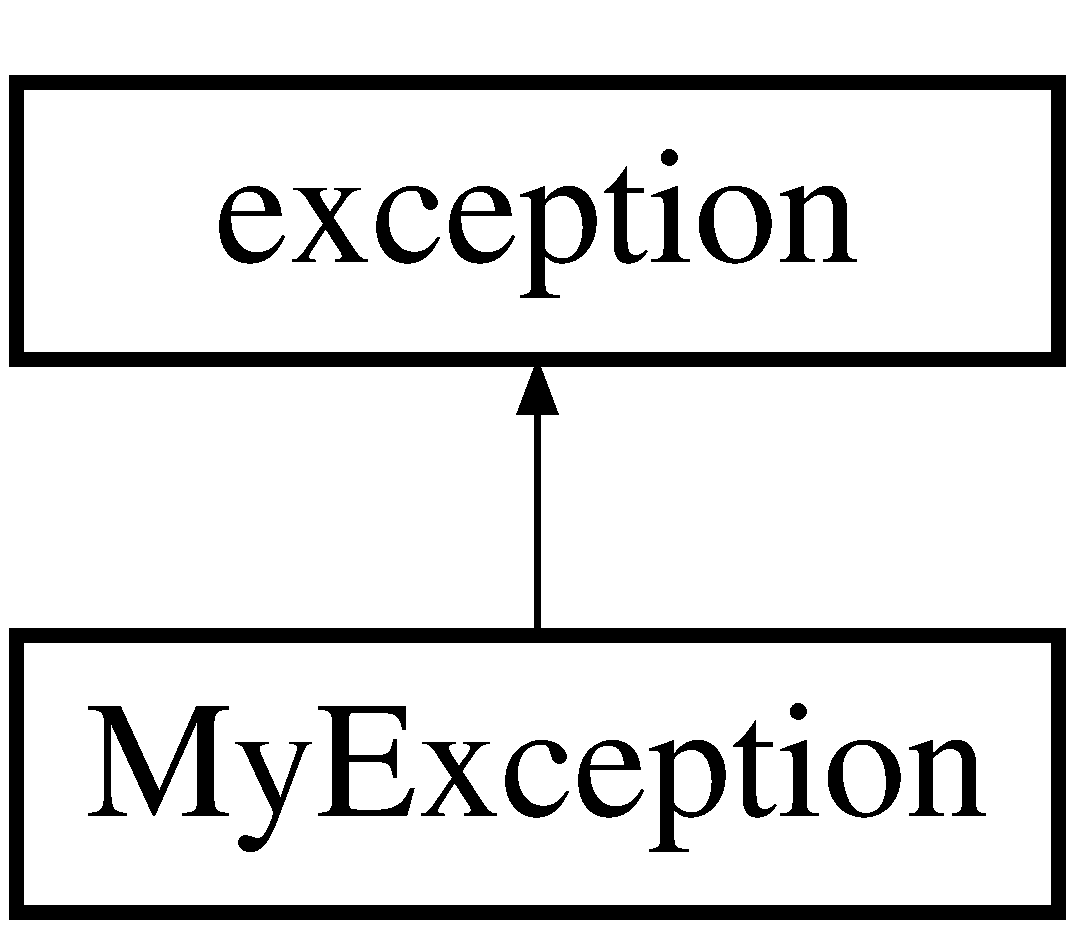
\includegraphics[height=2.000000cm]{class_my_exception}
\end{center}
\end{figure}
\subsection*{Typy publiczne}
\begin{DoxyCompactItemize}
\item 
enum \mbox{\hyperlink{class_my_exception_afe903d4d9fbfe77ff37010b2c191d4b9}{type}} \{ {\bfseries File\+Does\+Not\+Exist}, 
{\bfseries Errors\+In\+Input\+File}, 
{\bfseries Incorect\+Parameters}
 \}
\end{DoxyCompactItemize}
\subsection*{Metody publiczne}
\begin{DoxyCompactItemize}
\item 
\mbox{\hyperlink{class_my_exception_ab685f085f715db8734adad09b4b91874}{My\+Exception}} (\mbox{\hyperlink{class_my_exception_afe903d4d9fbfe77ff37010b2c191d4b9}{type}} typ, const string \&msg)
\item 
virtual const char $\ast$ \mbox{\hyperlink{class_my_exception_a2b3349cb98dbce0294df0e28f344877c}{what}} () const  throw ()
\end{DoxyCompactItemize}
\subsection*{Atrybuty publiczne}
\begin{DoxyCompactItemize}
\item 
string \mbox{\hyperlink{class_my_exception_a06a5c968d176fc702cdbe024207ddeef}{error\+Message}}
\end{DoxyCompactItemize}


\subsection{Opis szczegółowy}
Klasa obs�uguj�ca b�edy 

\subsection{Dokumentacja składowych wyliczanych}
\mbox{\Hypertarget{class_my_exception_afe903d4d9fbfe77ff37010b2c191d4b9}\label{class_my_exception_afe903d4d9fbfe77ff37010b2c191d4b9}} 
\index{My\+Exception@{My\+Exception}!type@{type}}
\index{type@{type}!My\+Exception@{My\+Exception}}
\subsubsection{\texorpdfstring{type}{type}}
{\footnotesize\ttfamily enum \mbox{\hyperlink{class_my_exception_afe903d4d9fbfe77ff37010b2c191d4b9}{My\+Exception\+::type}}}

Typ enum okre�laj�cy rodzaj b�edu 

\subsection{Dokumentacja konstruktora i destruktora}
\mbox{\Hypertarget{class_my_exception_ab685f085f715db8734adad09b4b91874}\label{class_my_exception_ab685f085f715db8734adad09b4b91874}} 
\index{My\+Exception@{My\+Exception}!My\+Exception@{My\+Exception}}
\index{My\+Exception@{My\+Exception}!My\+Exception@{My\+Exception}}
\subsubsection{\texorpdfstring{My\+Exception()}{MyException()}}
{\footnotesize\ttfamily My\+Exception\+::\+My\+Exception (\begin{DoxyParamCaption}\item[{\mbox{\hyperlink{class_my_exception_afe903d4d9fbfe77ff37010b2c191d4b9}{type}}}]{typ,  }\item[{const string \&}]{msg }\end{DoxyParamCaption})}

Konstruktor klasy 
\begin{DoxyParams}{Parametry}
{\em rodzaj} & b��du \\
\hline
{\em szczeg�y} & b��du \\
\hline
\end{DoxyParams}


\subsection{Dokumentacja funkcji składowych}
\mbox{\Hypertarget{class_my_exception_a2b3349cb98dbce0294df0e28f344877c}\label{class_my_exception_a2b3349cb98dbce0294df0e28f344877c}} 
\index{My\+Exception@{My\+Exception}!what@{what}}
\index{what@{what}!My\+Exception@{My\+Exception}}
\subsubsection{\texorpdfstring{what()}{what()}}
{\footnotesize\ttfamily const char $\ast$ My\+Exception\+::what (\begin{DoxyParamCaption}{ }\end{DoxyParamCaption}) const throw  ) \hspace{0.3cm}{\ttfamily [virtual]}}

Funkcja zwracaj�ca informacje o b�edzie 

\subsection{Dokumentacja atrybutów składowych}
\mbox{\Hypertarget{class_my_exception_a06a5c968d176fc702cdbe024207ddeef}\label{class_my_exception_a06a5c968d176fc702cdbe024207ddeef}} 
\index{My\+Exception@{My\+Exception}!error\+Message@{error\+Message}}
\index{error\+Message@{error\+Message}!My\+Exception@{My\+Exception}}
\subsubsection{\texorpdfstring{error\+Message}{errorMessage}}
{\footnotesize\ttfamily string My\+Exception\+::error\+Message}

Zawiera wiadomo�� informuj�c� o b��dzie 

Dokumentacja dla tej klasy została wygenerowana z plików\+:\begin{DoxyCompactItemize}
\item 
My\+Exception.\+h\item 
My\+Exception.\+cpp\end{DoxyCompactItemize}

\hypertarget{struct_odcinek_trasy}{}\section{Dokumentacja struktury Odcinek\+Trasy}
\label{struct_odcinek_trasy}\index{Odcinek\+Trasy@{Odcinek\+Trasy}}


{\ttfamily \#include $<$pch.\+h$>$}

\subsection*{Atrybuty publiczne}
\begin{DoxyCompactItemize}
\item 
\mbox{\hyperlink{struct_miasto}{Miasto}} $\ast$ \mbox{\hyperlink{struct_odcinek_trasy_ab5690824126c6707ef3e81e9b188728d}{miastoA}} = nullptr
\item 
\mbox{\hyperlink{struct_miasto}{Miasto}} $\ast$ \mbox{\hyperlink{struct_odcinek_trasy_aaa3d3e796a9673169d6f9c83c76af8b4}{miastoB}} = nullptr
\item 
int \mbox{\hyperlink{struct_odcinek_trasy_aa32dc6880fd7a9ed73d32d3f7c7f7e70}{odleglosc}} = 0
\end{DoxyCompactItemize}


\subsection{Opis szczegółowy}
Struktura zawierająca dane na temat odcinka wytyczanej trasy pomiedzy dwoma miastami 

\subsection{Dokumentacja atrybutów składowych}
\mbox{\Hypertarget{struct_odcinek_trasy_ab5690824126c6707ef3e81e9b188728d}\label{struct_odcinek_trasy_ab5690824126c6707ef3e81e9b188728d}} 
\index{Odcinek\+Trasy@{Odcinek\+Trasy}!miastoA@{miastoA}}
\index{miastoA@{miastoA}!Odcinek\+Trasy@{Odcinek\+Trasy}}
\subsubsection{\texorpdfstring{miastoA}{miastoA}}
{\footnotesize\ttfamily \mbox{\hyperlink{struct_miasto}{Miasto}}$\ast$ Odcinek\+Trasy\+::miastoA = nullptr}

wskaźnik na miasto początkowe \mbox{\Hypertarget{struct_odcinek_trasy_aaa3d3e796a9673169d6f9c83c76af8b4}\label{struct_odcinek_trasy_aaa3d3e796a9673169d6f9c83c76af8b4}} 
\index{Odcinek\+Trasy@{Odcinek\+Trasy}!miastoB@{miastoB}}
\index{miastoB@{miastoB}!Odcinek\+Trasy@{Odcinek\+Trasy}}
\subsubsection{\texorpdfstring{miastoB}{miastoB}}
{\footnotesize\ttfamily \mbox{\hyperlink{struct_miasto}{Miasto}}$\ast$ Odcinek\+Trasy\+::miastoB = nullptr}

wskaźnik na miasto końcowe \mbox{\Hypertarget{struct_odcinek_trasy_aa32dc6880fd7a9ed73d32d3f7c7f7e70}\label{struct_odcinek_trasy_aa32dc6880fd7a9ed73d32d3f7c7f7e70}} 
\index{Odcinek\+Trasy@{Odcinek\+Trasy}!odleglosc@{odleglosc}}
\index{odleglosc@{odleglosc}!Odcinek\+Trasy@{Odcinek\+Trasy}}
\subsubsection{\texorpdfstring{odleglosc}{odleglosc}}
{\footnotesize\ttfamily int Odcinek\+Trasy\+::odleglosc = 0}

Odległość pomięzdy dwoma miastami 

Dokumentacja dla tej struktury została wygenerowana z pliku\+:\begin{DoxyCompactItemize}
\item 
pch.\+h\end{DoxyCompactItemize}

\hypertarget{struct_trasa}{}\section{Dokumentacja struktury Trasa}
\label{struct_trasa}\index{Trasa@{Trasa}}


{\ttfamily \#include $<$pch.\+h$>$}

\subsection*{Atrybuty publiczne}
\begin{DoxyCompactItemize}
\item 
string \mbox{\hyperlink{struct_trasa_ab7c0cbfac427d219304c268ed1619cf9}{miastoA}}
\item 
string \mbox{\hyperlink{struct_trasa_a007c4abb2e5790f364766d3e8faa57d2}{miastoB}}
\item 
\mbox{\hyperlink{class_lista}{Lista}}$<$ \mbox{\hyperlink{struct_odcinek_trasy}{Odcinek\+Trasy}} $>$ \mbox{\hyperlink{struct_trasa_a187b2dcd9d158f54b549e15a1b12ff02}{trasa}}
\item 
\mbox{\hyperlink{class_lista}{Lista}}$<$ \mbox{\hyperlink{struct_odcinek_trasy}{Odcinek\+Trasy}} $>$ \mbox{\hyperlink{struct_trasa_addd78216be21eac061f507eb653a05b5}{mozliwa\+Trasa}}
\item 
int \mbox{\hyperlink{struct_trasa_adb6dfc9c3a7206f45d21cbdb1d02ae35}{dlugosc}} = 0
\item 
int \mbox{\hyperlink{struct_trasa_ad2cc10d999b3728f994a98dbfd447c6a}{mozliwa\+Dlugosc}} = 0
\end{DoxyCompactItemize}


\subsection{Opis szczegółowy}
Struktura zawierająca dane na temat wytyczanej trasy pomiędzy miastami 

\subsection{Dokumentacja atrybutów składowych}
\mbox{\Hypertarget{struct_trasa_adb6dfc9c3a7206f45d21cbdb1d02ae35}\label{struct_trasa_adb6dfc9c3a7206f45d21cbdb1d02ae35}} 
\index{Trasa@{Trasa}!dlugosc@{dlugosc}}
\index{dlugosc@{dlugosc}!Trasa@{Trasa}}
\subsubsection{\texorpdfstring{dlugosc}{dlugosc}}
{\footnotesize\ttfamily int Trasa\+::dlugosc = 0}

Odleglość z miastaA do miastaB \mbox{\Hypertarget{struct_trasa_ab7c0cbfac427d219304c268ed1619cf9}\label{struct_trasa_ab7c0cbfac427d219304c268ed1619cf9}} 
\index{Trasa@{Trasa}!miastoA@{miastoA}}
\index{miastoA@{miastoA}!Trasa@{Trasa}}
\subsubsection{\texorpdfstring{miastoA}{miastoA}}
{\footnotesize\ttfamily string Trasa\+::miastoA}

Nazwa miasta początkowego \mbox{\Hypertarget{struct_trasa_a007c4abb2e5790f364766d3e8faa57d2}\label{struct_trasa_a007c4abb2e5790f364766d3e8faa57d2}} 
\index{Trasa@{Trasa}!miastoB@{miastoB}}
\index{miastoB@{miastoB}!Trasa@{Trasa}}
\subsubsection{\texorpdfstring{miastoB}{miastoB}}
{\footnotesize\ttfamily string Trasa\+::miastoB}

Nazwa miasto końcowego \mbox{\Hypertarget{struct_trasa_ad2cc10d999b3728f994a98dbfd447c6a}\label{struct_trasa_ad2cc10d999b3728f994a98dbfd447c6a}} 
\index{Trasa@{Trasa}!mozliwa\+Dlugosc@{mozliwa\+Dlugosc}}
\index{mozliwa\+Dlugosc@{mozliwa\+Dlugosc}!Trasa@{Trasa}}
\subsubsection{\texorpdfstring{mozliwa\+Dlugosc}{mozliwaDlugosc}}
{\footnotesize\ttfamily int Trasa\+::mozliwa\+Dlugosc = 0}

Możliwa odleglość z miastaA do miastaB \mbox{\Hypertarget{struct_trasa_addd78216be21eac061f507eb653a05b5}\label{struct_trasa_addd78216be21eac061f507eb653a05b5}} 
\index{Trasa@{Trasa}!mozliwa\+Trasa@{mozliwa\+Trasa}}
\index{mozliwa\+Trasa@{mozliwa\+Trasa}!Trasa@{Trasa}}
\subsubsection{\texorpdfstring{mozliwa\+Trasa}{mozliwaTrasa}}
{\footnotesize\ttfamily \mbox{\hyperlink{class_lista}{Lista}}$<$\mbox{\hyperlink{struct_odcinek_trasy}{Odcinek\+Trasy}}$>$ Trasa\+::mozliwa\+Trasa}

\mbox{\hyperlink{class_lista}{Lista}} możliwych odcinków trasy (pomocnicza) \mbox{\Hypertarget{struct_trasa_a187b2dcd9d158f54b549e15a1b12ff02}\label{struct_trasa_a187b2dcd9d158f54b549e15a1b12ff02}} 
\index{Trasa@{Trasa}!trasa@{trasa}}
\index{trasa@{trasa}!Trasa@{Trasa}}
\subsubsection{\texorpdfstring{trasa}{trasa}}
{\footnotesize\ttfamily \mbox{\hyperlink{class_lista}{Lista}}$<$\mbox{\hyperlink{struct_odcinek_trasy}{Odcinek\+Trasy}}$>$ Trasa\+::trasa}

\mbox{\hyperlink{class_lista}{Lista}} odcinków trasy 

Dokumentacja dla tej struktury została wygenerowana z pliku\+:\begin{DoxyCompactItemize}
\item 
pch.\+h\end{DoxyCompactItemize}

%--- End generated contents ---

% Index
\backmatter
\newpage
\phantomsection
\clearemptydoublepage
\addcontentsline{toc}{chapter}{Indeks}
\printindex

\end{document}
